\graphicspath{{./assets/}}
\setcounter{mtc}{5}
\chapter{3rd Sprint: Resource provisioning  }
\fancyhead[R]{\ungaramond\small\textbf{Chapter V.  3rd Sprint: Resource provisioning  }}

\minitoc
\newpage
\section*{Introduction}

\section{Sprint Backlog}

\begin{longtable}[H]{|m{1.5cm}|m{3cm}|m{1.5cm}|m{8cm}|}
\hline
{\textbf{Epic ID}} & {\textbf{Epic}} & {\textbf{Story ID}} & {\textbf{Story}}\\
\hline
1  & \raggedright Provisioning resources using IaC playbooks and HCP config files.  &  1.1	 & Preparing provider specific(ovh) terraform config. \\
\cline{3-4}
& & 1.2 & Preparing ansible playbook to initiate provisioning. \\
\cline{3-4}
& & 1.3	& Setting up IaC host machine.  \\
\cline{3-4}
& & 1.4	& Cloud provider account and project creation.  \\
\hline
\caption{Table 3rd Sprint Backlog}
\end{longtable}

% \begin{longtable}[H]{|m{1.5cm}|m{3cm}|m{1.5cm}|m{8cm}|}
% \hline
% \multicolumn{1}{|c|}{\textbf{Epic ID}} & \multicolumn{1}{|c|}{\textbf{Epic}} & \multicolumn{1}{|c|}{\textbf{Story ID}} & \multicolumn{1}{|c|}{\textbf{Story}}\\
% \hline
% \endfirsthead
% \endhead
% \multirow{4}{*}{\textbf{1}}  & \multirow{4}{*}{Provisioning resources using IaC playbooks and HCP config files.} & 1.1 & \begin{tabular}[c]{@{}l@{}}Preparing provider specific(ovh) terraform config. \end{tabular} \\
% \cline{3-4}
% & & 1.2 & \begin{tabular}[c]{@{}l@{}}Preparing ansible playbook to initiate provisioning.\end{tabular}  \\
% \cline{3-4}
% & & \begin{tabular}[c]{@{}l@{}}1.3	\end{tabular} & \begin{tabular}[c]{@{}l@{}}Setting up IaC host machine. \end{tabular}  \\
% \cline{3-4}
% & & \begin{tabular}[c]{@{}l@{}}1.4\end{tabular} 	& \begin{tabular}[c]{@{}l@{}}Cloud provider account and project creation. \end{tabular}  \\
% \hline
% \caption{Table 3rd Sprint Backlog}
% \end{longtable}

\section{UML design : class diagram for cloud infrastructure }

\begin{figure}[H]\centering
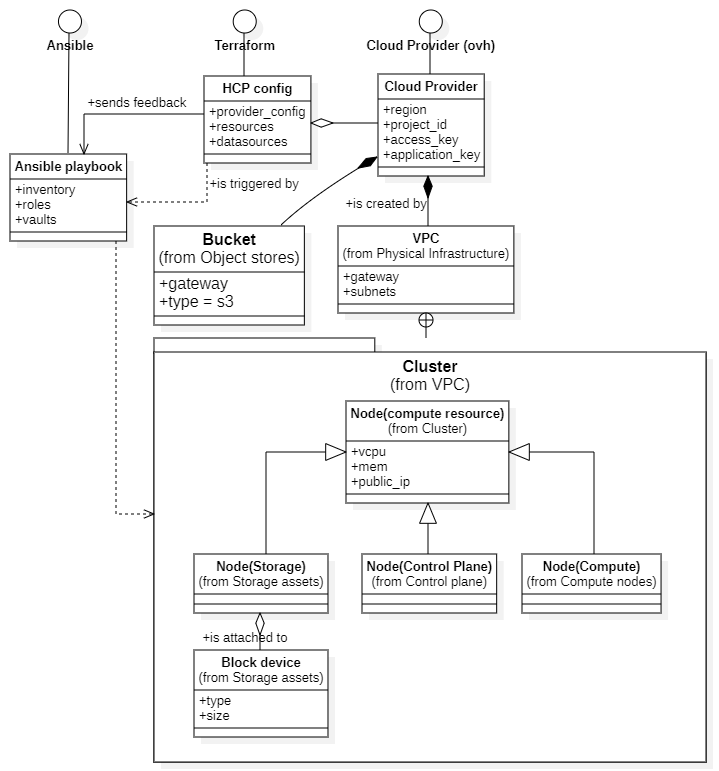
\includegraphics[width=1.0\textwidth,angle=00]{assets/f13.png}
\caption{Class Diagram for cloud infrastructure}
\label{fig:fig13}
\end{figure}

\section{“HCP config” diagram for cloud provisioning: }
The following figure illustrates the main resources declared in our terraform “HCP config”: 

\begin{figure}[H]\centering
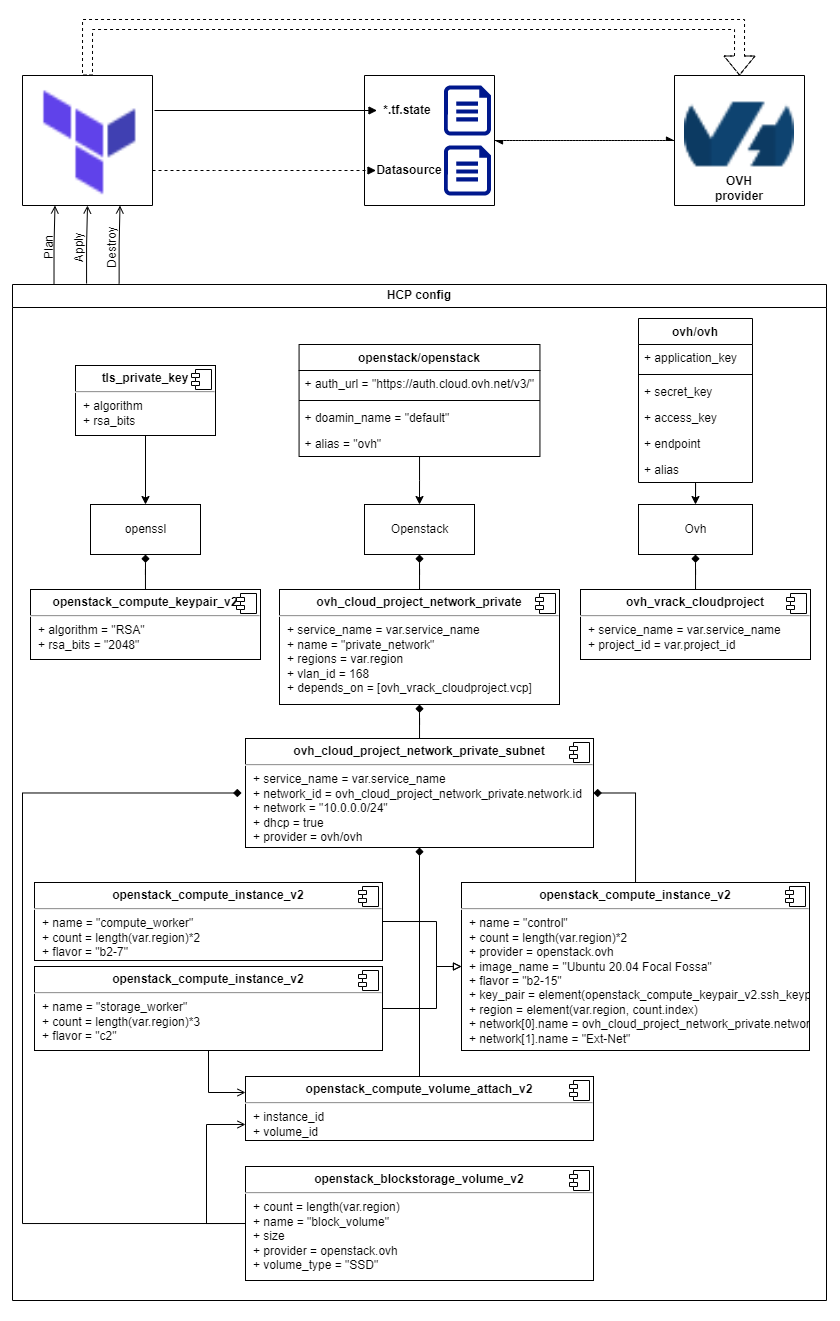
\includegraphics[width=1.0\textwidth]{assets/f14.png}
\caption{Diagram for cloud provisionning}
\label{fig:fig14}
\end{figure}

\section{Component diagram of provisioned resources}
\begin{figure}[H]\centering
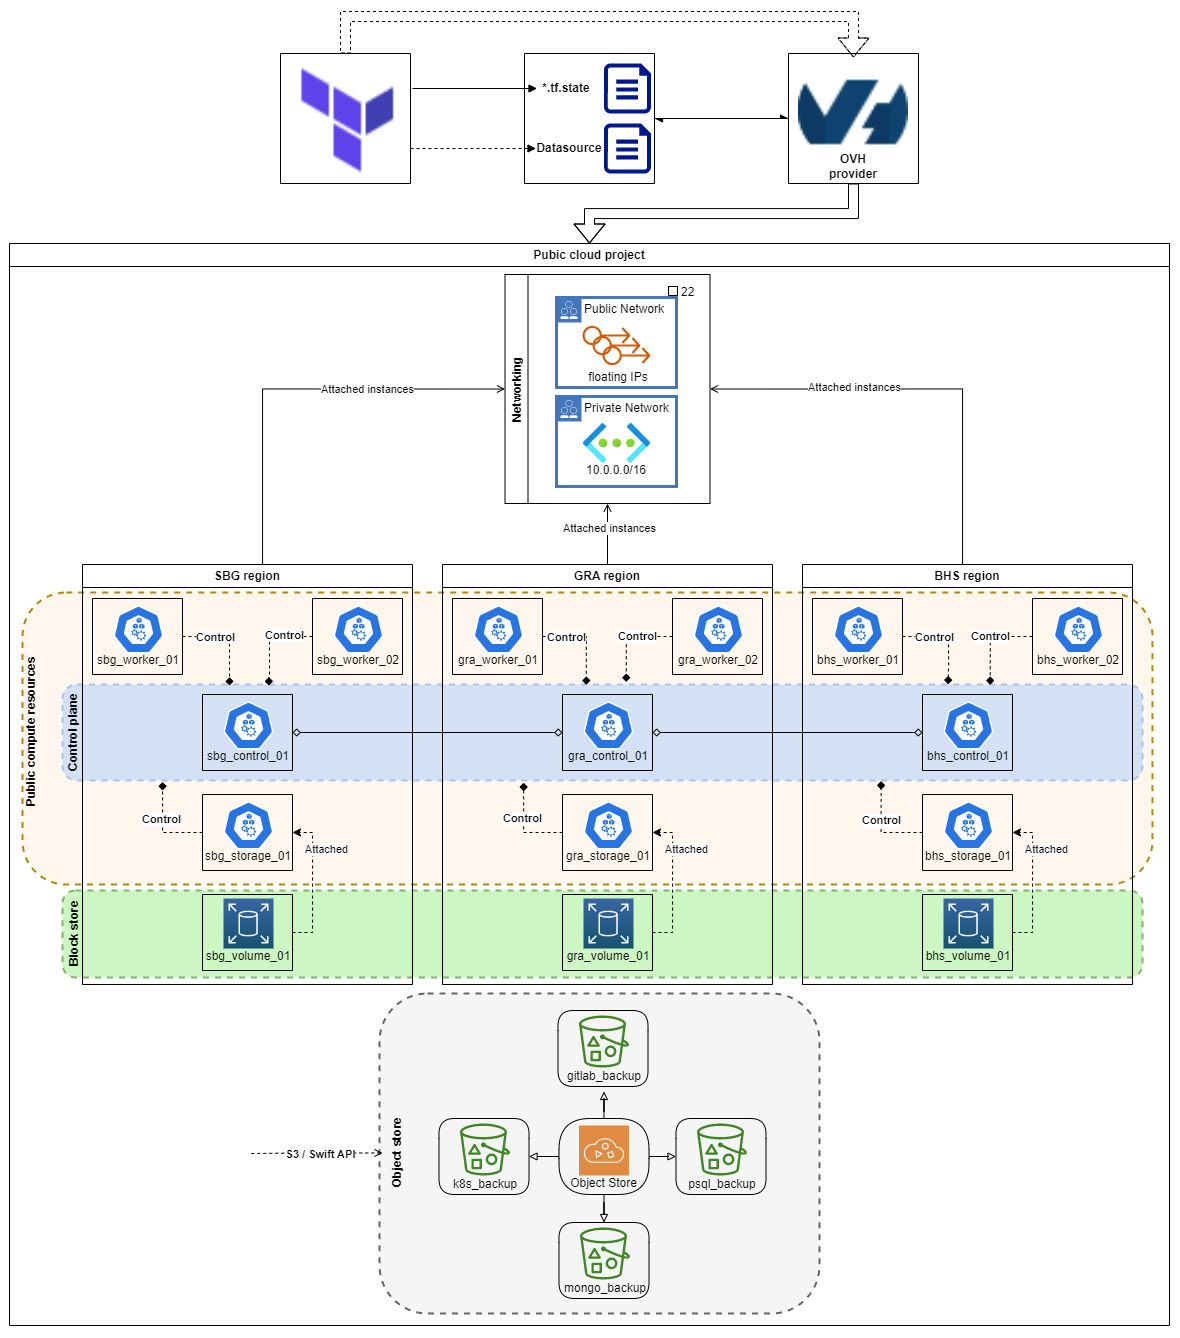
\includegraphics[width=1.0\textwidth,angle=00]{assets/f15.png}
\caption{Component diagram of provisioned resources}
\label{fig:fig15}
\end{figure}

The cluster resources were deployed to three regions. Namely, GRA, BHS, SBG. In each region, four instances were created. One of which will join the control plane, two will have the worker compute role and the last will have a second block device in raw format and will join the data storage backend. Various buckets from the object store will be provisioned and will serve as backup storage backends and high speed data storage.  



\section*{Conclusion}
